\section{Energy Auditing With Mobile Phones} 
\label{sec:mobileaudit}

Mobile phone penetration continues to rise in the United States and abroad.
As such, they serves as convenient interface between people and their environment.  
The combination of mobile network coverage and indoor wifi connectivity provides near-ubiquitous
connectivity at all times.  Coupled with the fact that mobile phones are personal devices that can serve as a proxy 
for the individuals, they provide a valuable point of interaction between the physical world, people, and
computation.  Through a combination of cloud technology, ubiquitious network access, and mobile phones, 
we can provide new ways to do in-situ diagnosis of opertional problems in the building, monitor personal energy consumption, 
and share related information with other occupants.  The phone becomes a lens through which we can directly observe the dynamics 
of our surroundings.

There are several systems challenges that must be overcome in order to achieve this vision.  Some can be solved easily 
through the primitives made available by StreamFS.  
%One of the 
% We need to place live metering on plug loads.  We need to integrate data from the BMS with plug load and other
% meter data.  We need to be able to approximate the attribution algorithms and tailor them for real-time processing.
We examine the challenges in capturing and maintaining a view of the physical world.  We track people and things,
deal with consistency management issues, and provide mechanisms for dealing with the occasional disconnection.
% \emph{Without addressing these systems issues, this vision cannot be achieved}.  
We deploy a number of
wireless power meters, use QR codes as a tagging mechanism, and build an android application that interacts directly with
StreamFS and plug-load devices.
% \subsection{Approach With StreamFS and Mobile Phones}
We use mobile phones to construct the entity-relationship 
graph of the locations, meters, and plug-loads in the building and use the processing features in StreamFS to provide detailed energy-attribution
statistics.  The `Mobile Energy Lens' uses QR-code sipe gesture to collect this information.  For example, if a computer is inside 
room Y and connected to meter Z, the user can register the computer, the room, and their ``is-in'' and ``attached-to'' relationships
explicitly through the a series of gestures that build the associated files and inter-relationships.  
We use these relationships to guide our analytics.
For example, the load curve of room Y consists of the sum of all the power traces for loads
inside room Y.  Our work examines \emph{three main challenges} in setting up and deploying a tag infrastructure through the building to 
support this application.

The first challenge is related to tracking.  Mobile phones present classical, fundamental challenges related to mobility.  Typically, mobility
refers to the phone, as the person carrying it moves from place to place.  However, in the energy-attribution
context, we refer to the movement of energy-consuming objects.  Tracking their relationships to spaces 
and people is as important as tracking people.  We describe how we deal with \emph{both moving people and 
moving objects} and show that these historically difficult problems can be addressed relatively easily, if the proper infrastructure 
and services are in place.  StreamFS plays an important role in offering the necessary services.
%We provide evidence that the approach is simple, incrementally deployable, and scalable.

The second challenge is about capturing the inter-relationship semantics and having these inform our analytics.
We adopt a general mechanism where physical tags identify objects in the world.  Our system uses \emph{QR codes} to tag things and locations 
in the building.  
% However, \emph{any tag that provides a unqiue identifier for an object could serve the same purpose}.
Once tagged, there are three types of swipe interactions -- 
registration, linking, and scanning -- which establish important relationships.  Registration is the act of creating a virtual object 
to represent a physical one.  Linking captures the relationship between pairs of objects.  Scanning is the act of performing an item lookup.
Each of these interactions requires a set of swipe gestures.  Linking requires two tag swipes while the other two actions
require a single tag swipe.  StreamFS conveniently already maintains an \emph{entity-relationship graph (ERG)} and we use it 
extensively in the Energy Lens to record things, people, and locations through these gestures.

The third challenge appears in dealing with indoor network connectivity and access.
In order to connect these components, we rely on `ubiquitous' network connectivity.  However, in practice, network
\emph{availability} is intermittent and our system must deal with the challenges of intermittency.  We discuss how caching
and logging are used to address these challenges.  Moreover, when connectivity is re-established, we must deal with
applying updates to StreamFS; updates recorded by the phone while disconnected.  
Conflicts may also occur during an update.  For example, the two updates may conflict about which items are attached
to which meters.  We implement a very simple conflict resolution scheme, described in section~\ref{sec:conflicts}.
Finally, physical state-transitions are represented as a set of updates to StreamFS that must be applied 
atomically.  However, StreamFS does not provide atomicity across multiple file operations.  We implement transactions through 
log-replay and transaction manager.  Our `Energy Lens' system is deployed in Sutardja Dai Hall at UC Bekreley.  We discuss
its architecture and design.  
  
% We also discuss novel strategies for tracking moving people/things and describe how we implement these in our system.  In summary, our work
% makes the following contributions:

% \begin{itemize}
% \item We design and implement a system that captures and combines physical entities, their inter-relationships, and real-time sensor data 
% 		in buildings.% using mobile phones, qr code, and a cloud-based infrastructure.
% \item We observe that certain combinations of swipes give us useful information to set the location of people and things over time.
% 		We codify this observation in our \emph{context-tracker} and use it to maintain consistency between the entity-relationship graph and the 
% 		state of the physical world.  To the best of our knowledge, this is radically different from the approaches in standard 
% 		localization techniques.  However, we argue that it can be used to \emph{enhance} their accuracy and overall performance.
% \item We implement a prefetching algorithm to obtain context-dependent information to both improve performance and
% 		enable disconnected operation.  We also design and implement a log-replay and transaction manager over our data management layer.  We describe how different conflict-resolution policies can be implemented and our rationale for the policies we chose.
% \end{itemize}

% \vspace{0.08in}

% In the next sections we go through a motivating scenario.  We then discuss some related work, followed 
% by the system architecture, evaluation, and future directions.


\section{Energy Lens Architecture and System Challenges}
The Energy Lens application aims to approximate the vision described in section~\ref{sec:elensvision}.  We tag
items with QR codes and allow users to 1) tag and register new items, 
2) tell us which meters are attached to which items, and 3) scan QR codes to view their load curve over a 
24-hour period.  Both individual items and spaces are scannable -- spaces present aggregate information
of the energy-consuming items within them.

The architecture consists of three layers: the sensing and tag layer, the data management and processing layer, and the application
layer.  In this section we discuss how aspects of each layer address the aforementioned challenges.
In deploying the application we run into various issues that inform our design.  
For example, \emph{QR code reading times vary substantially across phones
and lighting conditions}.  You must design for the least-common denominator in terms of camera quality and lighting.
Another aspect to consider is network access.  Within our building, although connectivity is mostly ubiquitous, network
access can be intermittent.  Network access may be unavailable for several reasons, including disassociation from an access point due
to idleness, dead spots in the building where connectivity to both wifi and 3G/4G are unavailable, multipath-induced
destructive interference, and various other reasons.  Dealing with these throughout the data collection and update phase is
especially troublesome.  We discuss mechanisms and algorithms for dealing with disconnected operation.

StreamFS serves as the data management and processing layer.  It must be \emph{extensibile} in order to add and remove
sensors and contextual information throughout the contextual capture process -- the collection of device inventory,
descriptive information, and associations between plug-loads and other items and locations in the deployment.
It must provide \emph{scalability} with the number of sensors and rooms in the building, since all the sensors produce periodic readings
and live, aggregate statistics is the main goal of the application.  Also, the application is interactive, so many mobile
phone users are constantly performing lookups.  StreamFS must handle these requirements.


\subsection{Challenge 1: Tracking People and Things}
\label{sec:tracking}

The Energy Lens application consists of a web application that displays timeseries data and an Android-based smartphone
app.
%Figure~\ref{fig:mobileapp} shows a few of screen shots from the application.  
The android app is relatively simple; consisting of a menu with only two options: Update deployment state, scan to view services.
Swipe gestures manipualte a local portion of the entity-relationship graph -- local with respect to a user's current location.
Since each location (room, floor) has a QR code attached to it and items are associated with those locations, we
can identify the location by name (\texttt{/buildings/SDH/spaces/4F/toaster}).  
Figure~\ref{fig:swipes} goes through the various sets 
of swipes.

\begin{figure*}[htb!]
\begin{center}
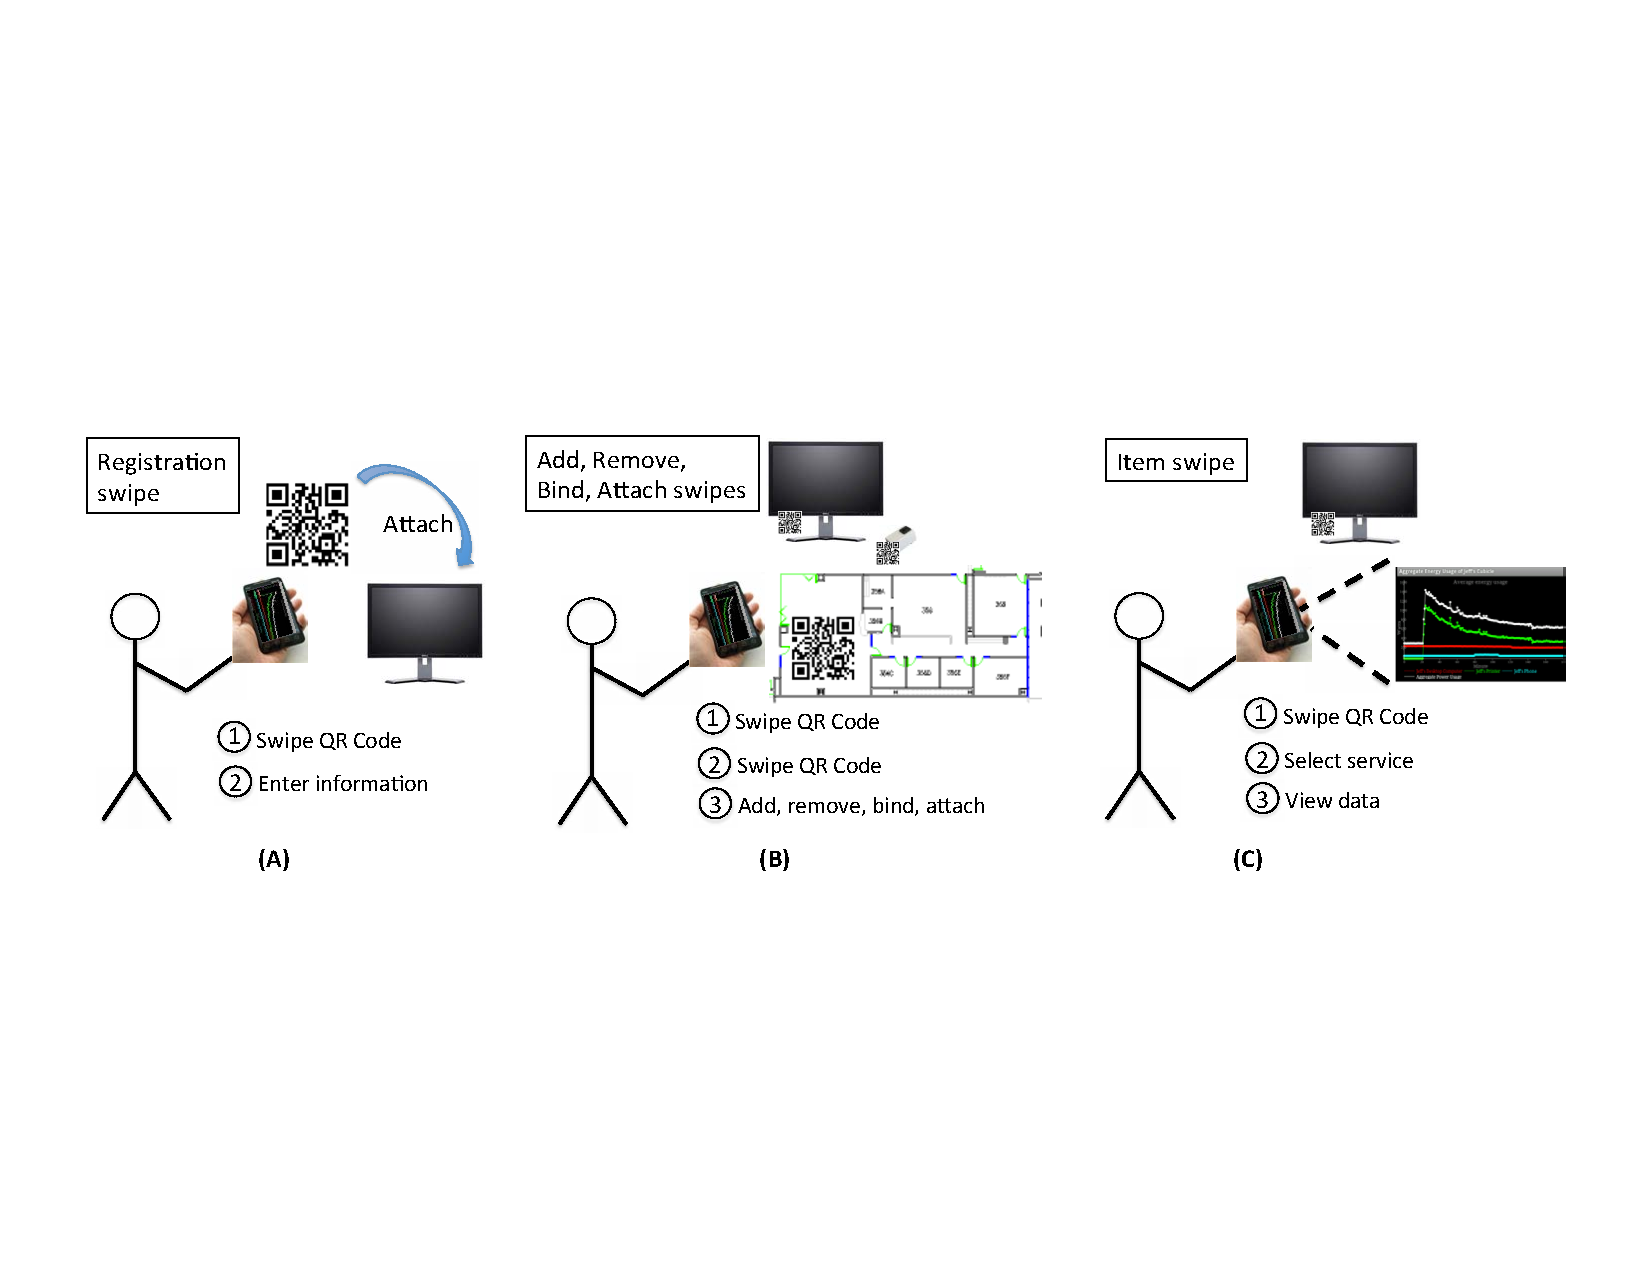
\includegraphics[width=0.8\textwidth]{figs/swipes}
\caption{Swiping gestures in the mobile application.  The registration swipe requires on a single swipe.  The 
linking and registration gestures require two swipes, and the look-up requires a single swipe.}
\label{fig:swipes}
\end{center}
\end{figure*}

The first set is called a `registration' swipe and we use it to register new items.  The user scans a QR code and the item it is \texttt{attached}
to.  This creates an `attached-to' link between them.  Adding, removing, binding, and attaching items is done with a pair of swipes.
A lookup is done with by swiping the QR code attached to an item.
% There are three major components in our architecture: QR codes, mobile phones, and StreamFS.

% How do we evaluate our ability to track people and things?
% This is a description evaluation.  We need to describe how the pieces interact.  What will fall out of the description is our strong dependence on occupants/users to give us information about the state of the physical world.  It’ll also fall out that what allows these pieces to fit together is network infrastructure.
We have designed a set of heuristics for setting the location during an update.  It piggybacks on the swipe gesture.
The following is a list of rules for automatically setting the location of people and things:

\begin{itemize}
\item When a user swipes at a location L, they are presumed to be at L for fixed period $\tau$.  An ``association timer'' is set to 
        release this association after $\tau$ seconds.
\item If the user swipes anything that is associated with a location $l$ at time $t \le \tau$, and $l(t)\ne$ L, 
        then we set the new location of the \emph{thing} they swiped to l(t) and reset the association timer.
\item If the user swipes anything at location l at time $t \ge \tau$, we set the location of the \emph{person} to l(t).
        We reset the association timer to $\tau$.
\item If a user registers a new location, they are presumed to be at that location.
\end{itemize}
\vspace{0.08in}


For each of these, we provide an interactive option to ask for location-change confirmation from the user.  So if we think the
user/item has moved but they have not, the preset action can be overridden.  The guiding principal we follow in our design
is to leverage the swipe gesture for as much contextual information as possible.  Furthermore, we do not explicitly track users.
Context is only set on the phone and used in operations sent to the server.  
We construct an entity relationship graph through 
naming in StreamFS.  StreamFS uses filesystem constructs, such as hierarchical naming and symbolic
links, which we use to express an acyclic relationship graph-structure.
%  which you are either editing directly or
% adding creating/destroying a relationship link in the graph.
Because location swipes give us direct confirmation of a user's location, it can be coupled with wifi localization mechanisms
and supervised learning algorithms to adjust the localization model as the user interacts with their environment. 
% For future work we intend to experiment with this mechanism.% to enable supervised-learning-based indoor wifi localization.

\subsubsection{Entity-Relationship Graph and Analytics}
We construct the entity relationship graph through naming in StreamFS.  StreamFS uses filesystem constructs, such as symbolic
links and hierarchical naming which are useful for expressing an acyclic graph structure (StreamFS checks for cycles when symlinks 
are created).  
The following general path-naming text patterns are used to express different portions of the ERG.
\texttt{/path/to/device\_or\_item}, 
\texttt{/path/to/qrc}, \texttt{/path/to/space}, \texttt{/path/to/taxonomy}, \texttt{/path/to/users}.  
Registered meters are placed in the device path, \texttt{/dev}.  Items are stored in \texttt{/inventory}.  QR codes are stored 
in \texttt{/qrc}.  When an item is registered a 
symbolic link is created from the specific qr code directory to the item.  \texttt{/spaces} contains a hierarchy of floors, rooms, 
and sub-spaces.  \texttt{/users} contains the list of usernames.  We also have a \texttt{/tax} directory, where we construct an
device hierarchy for access by plug-load category.  Placement (location) is also captured with symbolic links. 

Each hierarchy not only represents the physical relationships between items but also provides a structure for 
enabling hierarchical aggregation and querying.  We define a load-curve generating process called \texttt{loadcurve}, displayed in 
Listing~\ref{code:loadcurve_part}.  The full process job can be found in the Appendix, Listing~\ref{code:loadcurve_full}.

\begin{lstlisting}[caption={Partial load curve code used to generate aggregate load curves in the Energy Lens application.},label={code:loadcurve_part}]
function(buffer, state){
    var outObj = new Object();
    var timestamps = new Object();
    outObj.msg = 'processed';
    if(typeof state.slope == 'undefined'){
        state.slope = function(p1, p2){
            if(typeof p1 != 'undefined' && typeof p2 != 'undefined' &&
                typeof p1.value != 'undefined' && typeof p1.ts != 'undefined' &&
                typeof p2.value != 'undefined' && typeof p2.ts != 'undefined'){
                if(p1.ts == p2.ts)
                    return 'inf';
                return (p2.value-p1.value)/(p2.ts-p1.ts);
            }
            return 'error:undefined data point parameter';
        };
        state.intercept = function(slope,p1){
            if(typeof p1 != 'undefined' &&
                typeof p1.value != 'undefined' && typeof p1.ts != 'undefined'){
                return p1.value - (slope*p1.ts);
            }
            return 'error:undefined data point parameter';
        };
    }
}
\end{lstlisting}

When a new meter is measuring a device in a room, the Energy Lens app actives the \texttt{loadcurve} process through a general
subscription instance.  For example\\ \texttt{sub.source(/sdh/4F/473R/*).filter(unit:KW).destination(/sdh/4F/473R/lc\_324hb)}
creates a subscription for streams with the prefix specified in the source call with the filter on the metadata where 
the units produced on KW and pipes it into an instance of the \texttt{loadcurve} process.  Note \texttt{/sdh/4F/473R/lc\_324hb}
is a symbolic link to \texttt{/proc/loadcurve/324hb}, the instance file the represent the aggregator for this room.
The initial instance file can only be created if the source has a match.  The app checks if there are any streams in the room
every time a new meter is added.  If it is the first stream in the room, the pipe and corresponding symbolic link is created. 
If all the meters are removed from the room, the process is killed and the symlink becomes a dangling pointer that needs to
be cleaned up.  The cleanup is done by the Energy Lens application.  StreamFS does not provide a clean-up mechanism.



\subsection{Challenge 2: Consistency Management}
We use an eventual-consistency model for maintaining the ERG over time.  Naturally, the spatial inter-relationships
change over time as items are moved and replaced.  In order to deal with this we offer two options: 1) we periodically
re-scan the items and their locations, essentially re-capturing the inventory collection portion of the audit or
2) we allow building occupants to participate as auditors, capturing their own personal items and shared items.
This should provide at least as much value as a periodic energy audit and can be completed in a fraction of the 
time~\cite{aceee_mobileaudit}.

Placement (location) is captured with symbolic links as well.
Node types inform the application of the nature of the relationship.  We define five distinct types: item, meter, 
location, category, and tag.  The following relationships are constructed with symlinks between different node types:

\begin{itemize}
\item {\textbf Owned-by}: When a meter/item/location is tagged as belonging to a user.
\item {\textbf Bound-to}: When a meter is attached to an item and taking physical measurements associated with that 
		device, we say that the meter is ``bound-to'' the device.
\item {\textbf Attached-to}: When a meter/qr code/item is attached to another meter/qr code/item but \emph{not} taking any 
		physical measurements for that item, we say that the meter/item is ``attached-to'' the other meter/qr 
		code/item.  QR codes cannot not be attached to each other.
\item {\textbf Is-in}: When a meter/item is inside a location, we say that the meter/item ``is-in'' that location.
\item {\textbf Type-of}: When an item is labeled by as a known, specific, type, we say that the item is a ``type-of'' thing 
		specified by the its label.
\end{itemize}

All symlinks are interpreted based on these rules of association.  As items move, symlinks are removed and re-created
in a different folder.  We know your current location by following the path from the QR code directory, across a symlink, 
to a file in the space directory.  Items associated with a space have a floor or room folder point to the item
via a symlink.  This is how we record the location of things throughout the building.

\begin{figure}[htb!]
\begin{center}
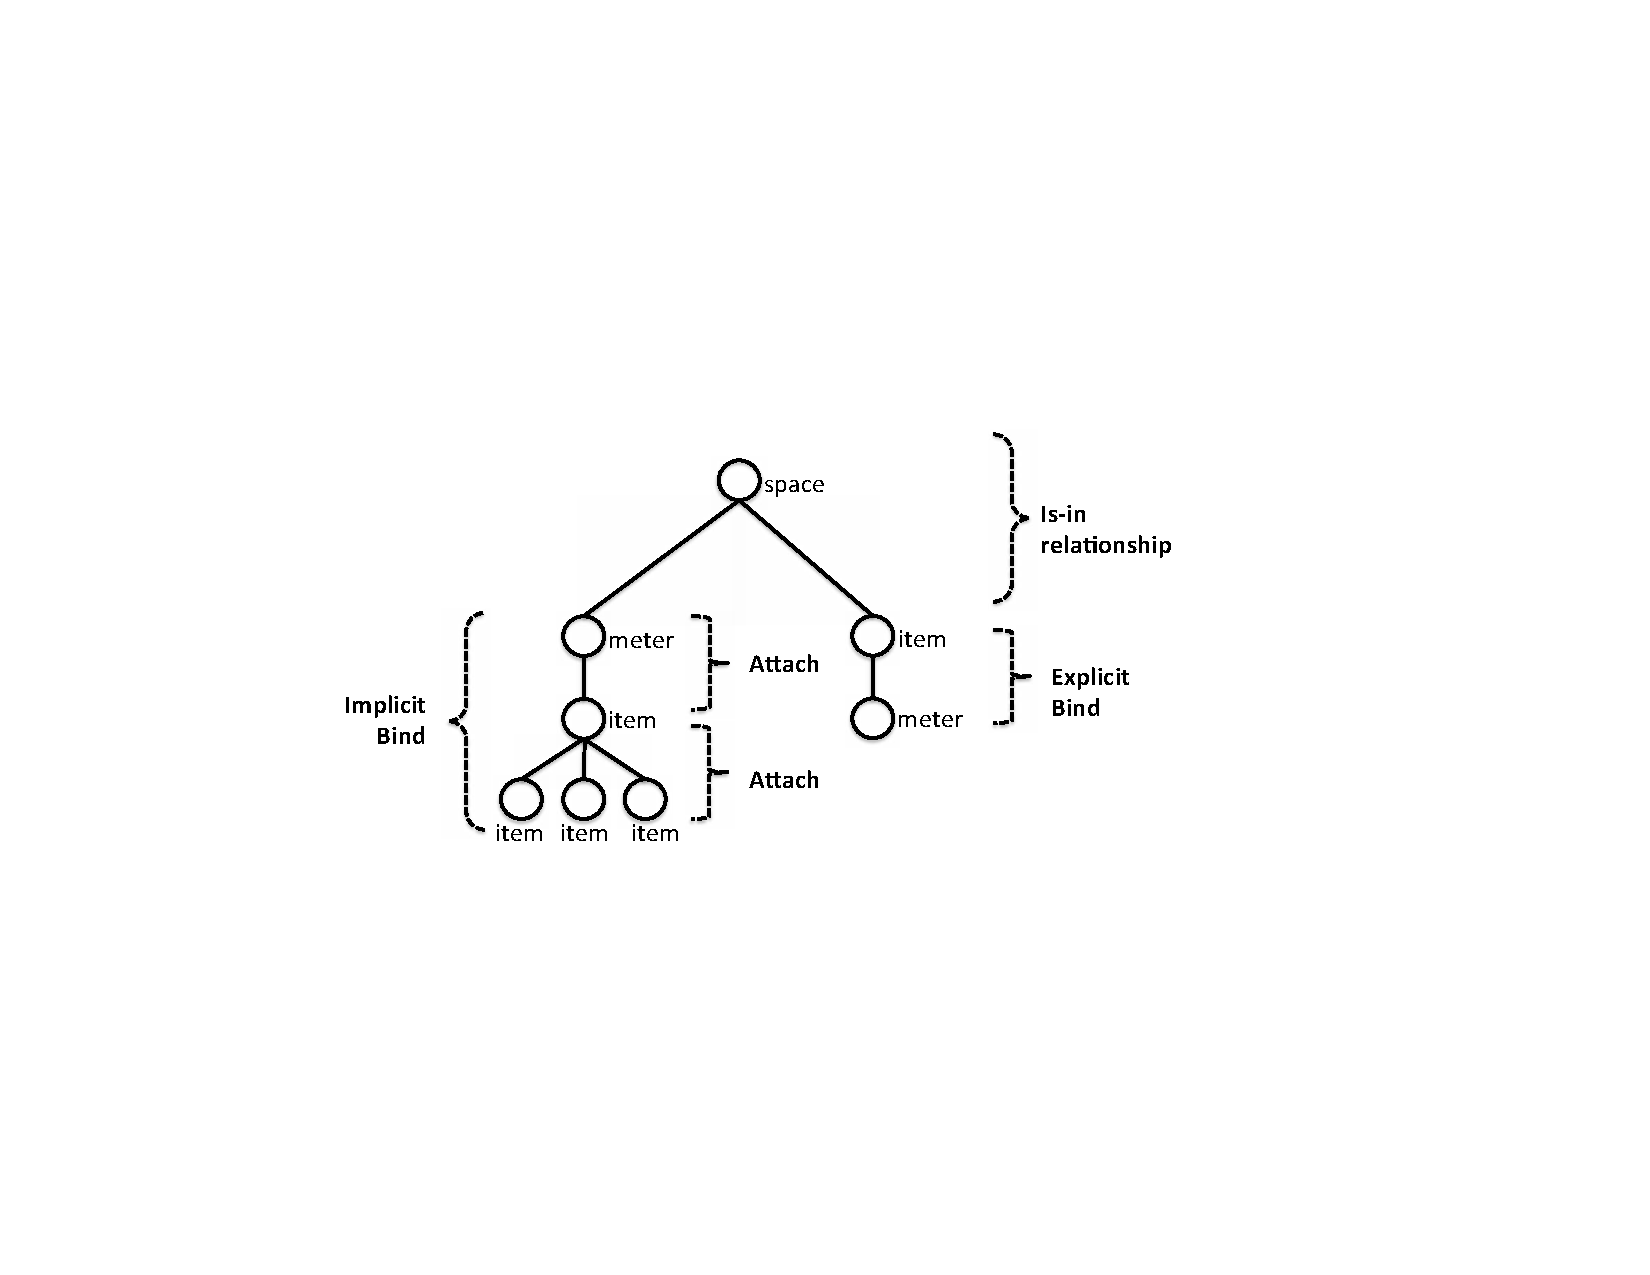
\includegraphics[scale=0.75]{figs/bindattachstructs}
\caption{This diagram shows the relationship capture between the objects and locations in the building for the 
energy audit application.  Children of a space node have an ``is-in'' relationship with the space.  An item
with another item as a child have a ``is-attached'' relationship and meters attached to items are bound to each other.
Note, this is a \emph{subset} of the relationship diagrams generated across our three applications.}
\label{fig:attachandbind}
\end{center}
\end{figure}





\subsection{Challenge 3: Disconnected Operation}
Although connectivity is ubiquitous, network access is not.  This occurs due to dead zones, 
idle-disconnect and failed hand-off between access points.  When encountered in practice, especially while editing
deployment state, it can be quite frustrating and discourage use of the application.  We designed a
mechanism that does smart caching, not only to improve performance, but also to allow for disconnected operation.

The Energy Lens application downloads a portion of the ERG when a user enters a new floor.  The application fetches the portion
of the graph rooted at the floor.  
Figure~\ref{fig:sdh_4f_erg} shows just a small portion of that entity-relationship graph for the floor we are monitoring in
our deployment.  
A prefetch populates the cache with all entity nodes on that floor, their associated metadata,
and 30 minutes of data from the stream entities.  The full fetch of the 4th floor data set includes
176 nodes and about 1 MB of meter data.  In total, the app downloads ~1.2 MB of data upon re-connection.
Prefetching allows users to continue interacting with the application as if they were still connected (as long as they remain on
the same floor).  Without it, the application is not functional until a network connection is established.

% \begin{algorithm}
% \caption{Prefetch Loop}
% \label{alg:prefetch}
% 	\begin{algorithmic}
% 	\While {true}
% 	\If {connected and active}
% 	    \State $req\gets [t_{i-n}, OP_R]$
% 	    \State $resp\gets $ send($req$)=$[t_{i-k}, OP_R],\dots, [t_{now}, OP_R]; $ 
% 	    \State $n >= k$
% 	    \For {$j = 1 \to size(resp)}$
% 	    	\State $op \gets$ $resp[j]=[t_{i-k+e}, OP_R]$
% 	    	\State apply($op$)
% 	    \EndFor
% 	\EndIf
% 	\If {active}
% 		\State Sleep for 10 minutes
% 	\Else
% 		\State Sleep for 1 hour
% 	\EndIf
% 	\EndWhile
% 	\end{algorithmic}
% \end{algorithm}

\begin{algorithm}[h!]
 \SetAlgoLined
  \While{1}{
	  \If{connected and active}{
	  	(1) $req\gets [t_{i-n}, OP_R]$\;
	  	(2) $resp\gets $ send($req$)=$[t_{i-k}, OP_R],\dots, [t_{now}, OP_R] $\;
	  	(3) $n >= k$\;
	  	\For{$j = 1 \to size(resp)$}{
	  		(1) $op \gets$ $resp[j]=[t_{i-k+e}, OP_R]$\;
	  		(2) apply($op$)\;
		}
	  }

	  \If {active}{
		(1) Sleep for 10 minutes\;
	 \Else{
		(1) Sleep for 1 hour}\;
	}
  }
 \caption{Prefetch Loop.}
 \label{alg:prefetch}
\end{algorithm}


The Energy Lens periodically syncs with StreamFS to obtain updates to the ERG and maintain a locally consistent view.  
Let $OP_R$ be an operation performed on the node rooted at node $R$ and $t_i$ be the current time on the phone.  
% Algorithm~\ref{alg:prefetch} shows the pseudo code for the prefetch process.  
After a set period, the phone sends the server
its last performed operation and the time that operation was performed.  The server responds with any operations that have
take place since then.  The client applies those operations internally to the cached version of the the ERG in order to 
maintain consistency.  The ``\emph{active}'' parameter-check, is for energy savings.  If the phone application is active, the
check occurs every 10 minutes, otherwise it occurs ever hour.

The process is demonstrated in Figure~\ref{fig:interactions}.  The components shown are the \emph{ERG cache}, the \emph{operation
log (OpLog)}, and the \emph{prefetcher}.  We separate the steps in the figure as a READ sequence and a WRITE sequence.
All reads go to the cache (steps 1 and 2 on the left hand side of the figure).  Writes go through the OpLog (steps 1 - 5 on the right
side of the figure).  For writes, 
the application makes a write request (1) and it is forwarded to StreamFS (2).  If StreamFS is reachable and the write is
successful (3), the operation is applied to the ERG cache (4) and the response is sent the application (5).
If the operation is not successfuly, step 4 is skipped.  If StreamFS could not be reached, step 3 is skipped, and the operation
is written to the OpLog.  The OpLog is flushed to the server, by the prefetcher, upon re-connection. 

The OpLog contains records of operations that are eventually applied to StreamFS.  Some of those operations
are actually groups of operations that need to be applied atomically.  For example, 
when a bind or attach operation occurs, we append the timestamp to the item(s) that are being connected, as well as create
a link between them in the graph.  The application uses both the link and the added metadata to fetch the appropriate
graph for display.  These operations must be applied atomically or not be applied at all.
When the log is dumped, the global transaction manager (GTXM) -- the layer that handles log dumps and transaction processing --
attempts to apply the log in timestamp order.


\begin{figure}[htb!]
\begin{center}
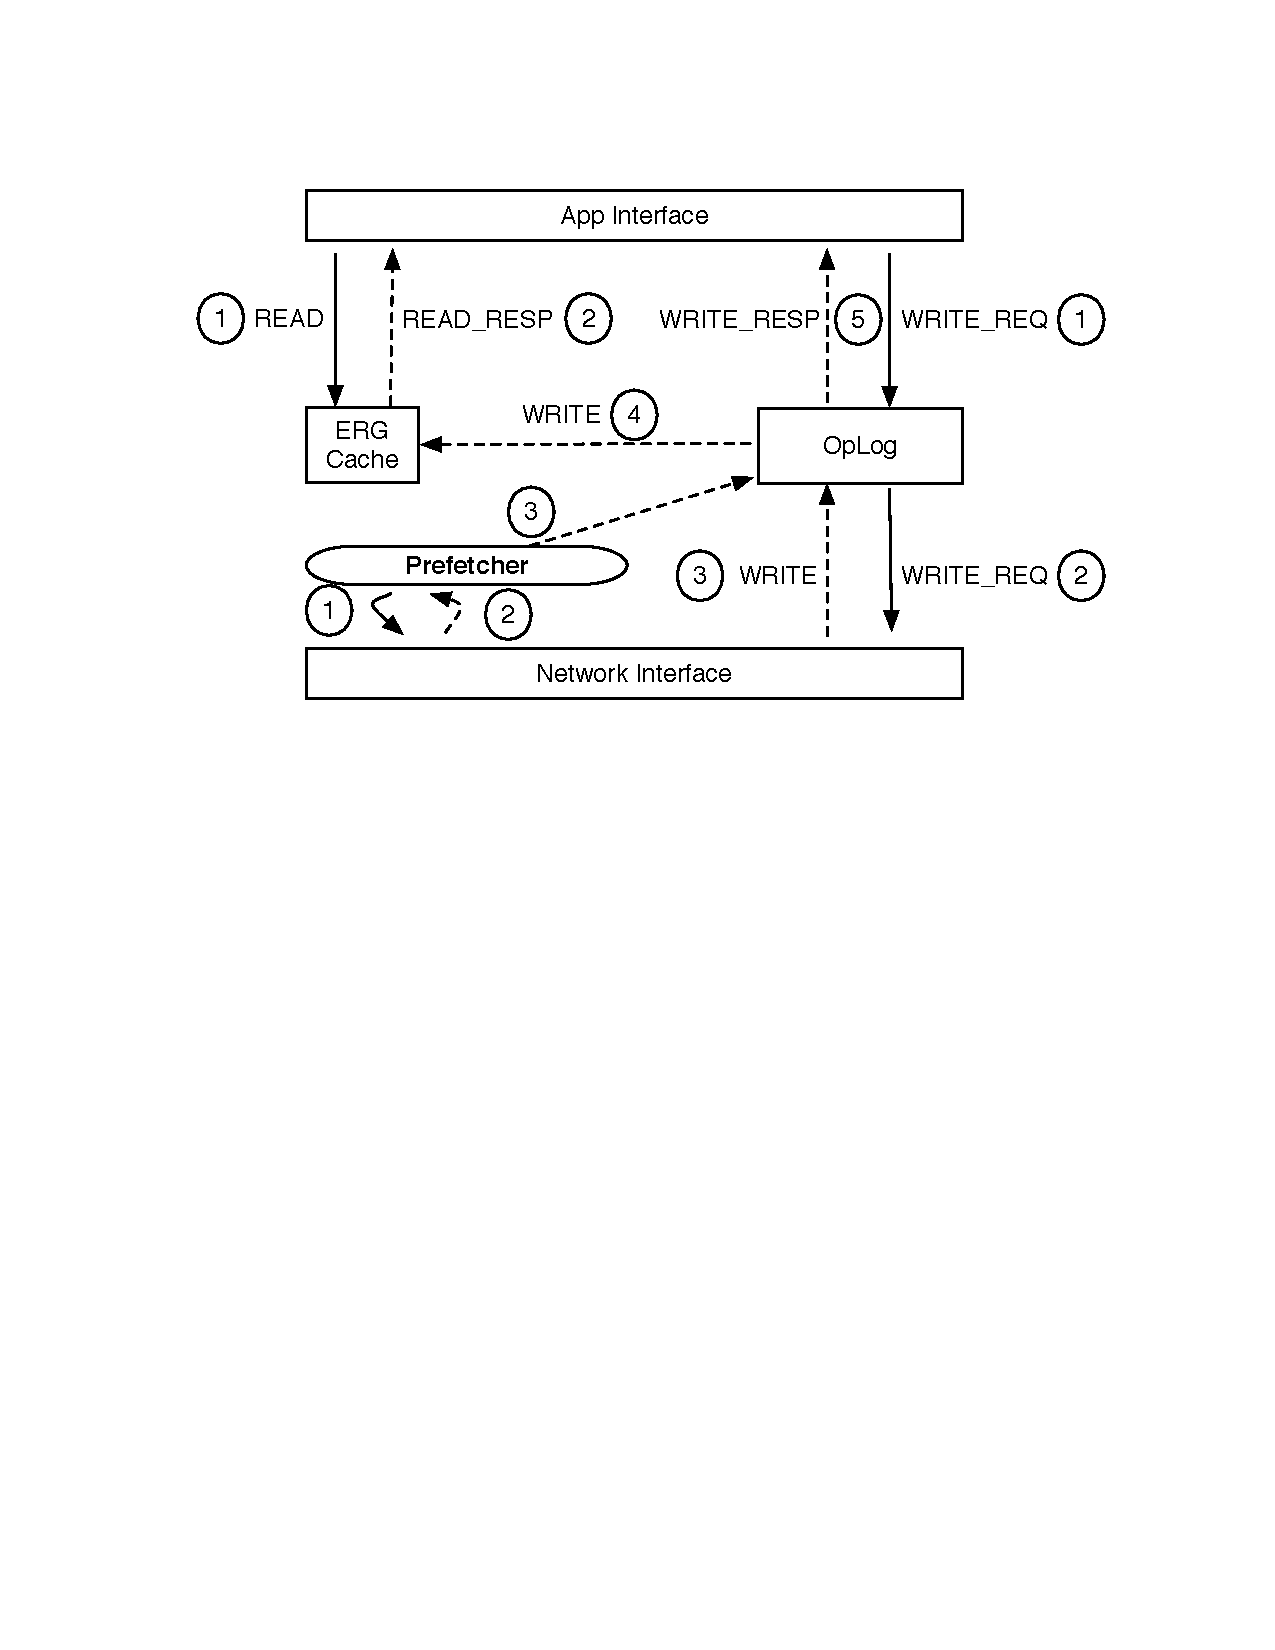
\includegraphics[scale=0.80]{figs/standard_interaction}
\caption{Standard mechanisms for consistency management on the phone.  All READ request go to the local
cached version of the ERG.  All WRITES must go through the OpLog.
They are eventually applied to the cache
if successful and logged if the StreamFS is unreachable.  These components are directly built into the 
Energy Lens application.}
\label{fig:interactions}
\end{center}
\end{figure}

\subsubsection{Log dumps and conflict resolution}
\label{sec:conflicts}
When the Energy Lens application is started it contacts the server and attains the server's local clock time. 
It notes its local time as being equal to the timestamp of the server and calculates all subsequent timestamps
using its local clock.  When an operation or transaction is added to the OpLog, a timestamp is appended.  Let $t_s$ be the timestamp 
on the server, $t_l$ be the timestamp on the phone when $t_s$ is recorded, and $t_{now}$ be the current time on the phone.  
Each operation/transaction is timestamped with $t_{approx}$ where:

\begin{equation}
t_{approx} = t_s + (t_{now} - t_l)
\end{equation}

This timestamp is a general approximation of when the operation should be applied on the server.  The server applies 
these is ascending timestamp order.

Generally, a conflict occurs if there is any operation or transaction that was applied after the timestamp of the current operation
being processed.  A typical transaction manager must rollback the state of the database, apply the operation, and replay
the log.  However, conflict resolution is much simpler in this context.  \emph{The latest operations reflect the state of the
world because they are updates induced by direct interaction with the world at that point in time.}  Therefore, if there is a conflict
between a set of operations, the old ones can all be discarded.

Operations that are discarded are done so silently.  We make failures silent for two reasons: 1) There is no way to contact the app when 
failure occurs.  Mobile phones
do not often have reversably reachable addresses.  2) Failure assumes the operation was based on a false assumption about the state
of the world.  


\section{Energy Lens Experience and Results}

Figure~\ref{fig:tsdata} shows three screen shots of power traces obtained from the ACme deployment, and displayed
through the Energy Lens.  Notice that there is
some data missing in the graph.  This occurs because of in the network transmission, reboots on the data management layer,
or failed scripts that are automatically restarted.  In all cases we get holes in the data.  To compute aggregates, interpolation 
is necessary.  StreamFS offers a real-time processing facility, whereby javascript operaters can be applied
to streaming data.  This allows us to clean it as it comes in and compute the aggregate traces.  We are currently experimenting
with various aggregation models to give occupants deeper insights.  


\subsection{Deployment Experience}
\label{sec:depexp}

% We deployed 20 ACme power meters~\cite{acmemeter} on a single floor of a building on campus.  The data was made available through
% sMAP~\cite{smap} and forwarded to our processing and data management layer, StreamFS.  
We distributed several ACmes~\cite{acmemeter} throughout a single floor in our building and registered various plug loads as being measured by them.  We also tagged
hundreds of items and locations throughout the entire building.  In total we tagged 20 meters, 20 metered items, 351 un-metered items,
 and 139 rooms over 7 floors.  Figure~\ref{fig:tsdata} shows three screen shots of power traces obtained from the ACme deployment, and displayed
 through the Energy Lens. 

\begin{figure}[htb!]
\begin{center}
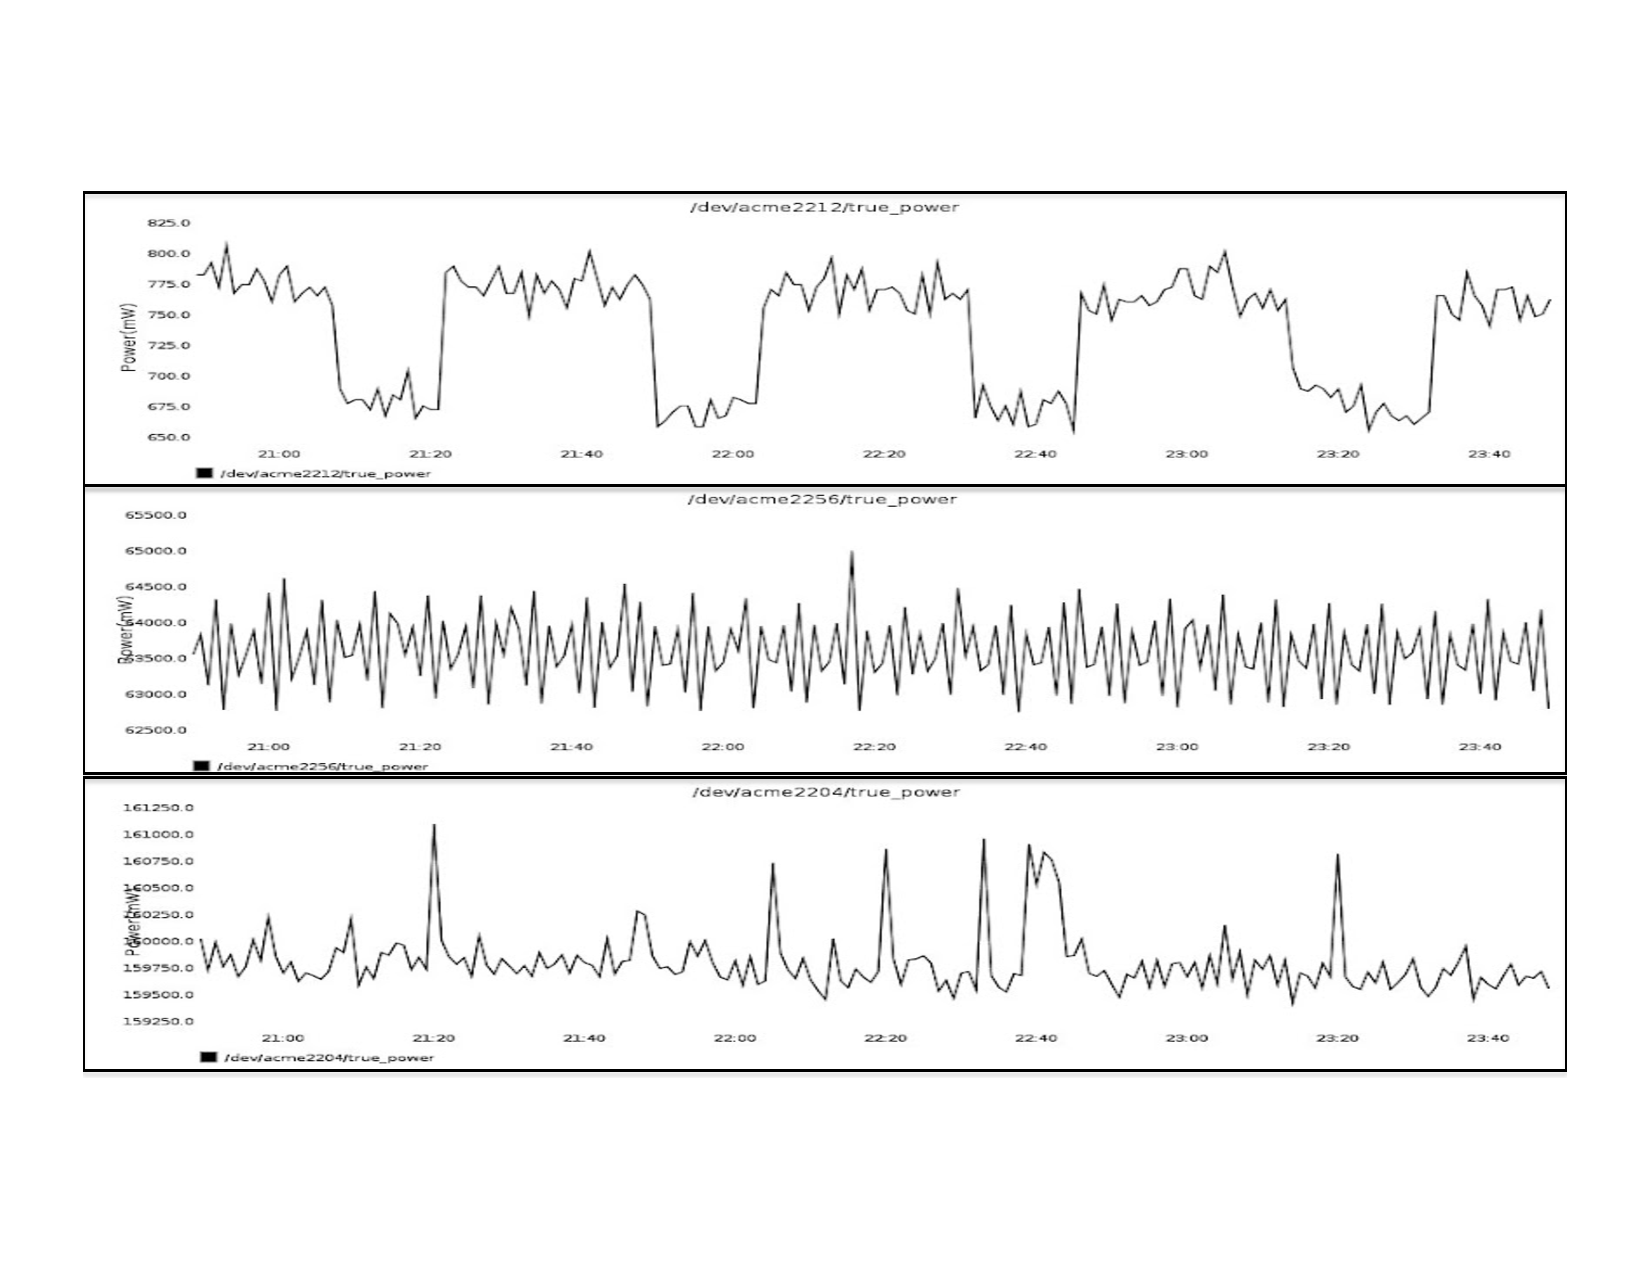
\includegraphics[scale=0.33]{figs/graphs_screen}
\caption{Power traces obtained from power meters attached to various plug load on one of the floors of
a building on campus.  These show screen shots of the Energy Lens timerseries data display.}
\label{fig:tsdata}
\end{center}
\end{figure}

In our initial deployment we found that the use of our tracking scheme to be effective, especially in conjunction with
interactive confirmation.  The ERG was effective at capturing deployment state, although highly mobile items, such as laptops,
were particularly difficult to keep track of.  Finally, our disconnected operation mechanism was effective at masking 
intermittent connectivity.  For future work we will baseline the floor's energy consumption before and after the deployment 
and measure if more visibility and analytics indeed motivates occupants to use less.

% \section{Acknowledgements}
% This work is support by the LoCal NSF Grant \#CPS-0932209 and ActionWebs NSF Grant \#CPS-0931843.  We would also like
% to thank Albert Goto for deployment help and Amazon for providing our computing infrastructure.

% Pub/sub architecture
% time decoupling
% variable time-decoupling achieved through the datastore as a buffer
% synchronization decoupling
% Either the publisher or subscriber run asynchronously.
% space decoupling
% The subscriber doesn’t have an explicit reference to the publisher.
% Programming model for real-time data
% Naming/tagging streams
% Dealing with dynamism through tagging
% Built-in functions for physical data
% heat modeling
% electrical modeling
% mathematical modeling

% Security and privacy
% Discussion.  Various topics related to StreamFS here.  Also some topics related to managing security in StreamFS for doing control.  Include another half page, perhaps.


% * Experiment that we need to run.\\
% ** Code that needs to be writexttten and experiment that needs to be run

\subsubsection{QR code design}
\label{sec:qrc}
Our choice to use QR codes is important, since the \emph{only way to scale -- in deployment size and management complexity -- is to
involve building occupants}. QR codes are cheap to produce.  They can be printed and attached to items with tape or sticky paper.  
Figure~\ref{fig:qrcexsecond} shows an example QR code used in our deployment.  These are placed on physical
objects and spaces throughout the building to link between the physical world and our virtual representation of it.

With the number of physical objects and places in a building, \emph{we must rely on the occupants
to scale our deployment and manage it}. Because QR codes are easy to produce, we provide occupants with a webpage that
that produces them.  They print them out, place them on items or places they want to interact with and use them to register
items in StreamFS through the Energy Lens.
Since occupants are our target users, we must make the application easy to use.  For QR code scan-times, vary by lighting conditions, 
camera quality, and hand movements.  In poor conditions scanning is cumbersome; ultimately de-motivating continued use.  
QR codes must be designed to minimize scanning time.  In our initial deployment and experiments we observe
that complex QR code code not only have an longer average scanning time but also experience a larger variance in scanning time.  
The more complex the pixel design in the QR code, the harder it is for the camera to focus and capture it. 

We scanned each QR code shown in Figure~\ref{fig:qrcexcomp}, under light and dark lighting conditions.  
Each experiment was run 10 times and Table~\ref{tab:qrscans} shows a statistical summary.  Scanning the simple QR code under well-lit 
conditions performed the best.  The complex QR code under  the same condition takes about 28-36\% longer to scan.
Perhaps even more important is the variance.  Notice that the variance with the simple QR code is smaller.
QR code image complexity increases with the amount of information you encode on it.  Therefore, it was important to decrease the
amount of information we encoded, \emph{placing the complexity in the lookup rather than the tag.}

% \begin{figure}[htb!]
% \begin{center}
% \subfigure[Long QR Code.]{%
%             \label{fig:qrcexfirst}
%             
\includegraphics[scale=0.148]{figs/qrcexlong}
%         }
% \subfigure[Minimized QR Code.]{%
%             \label{fig:qrcexsecond}
%             
\includegraphics[scale=0.35]{figs/qrcex}
%         }
% \end{center}
% \caption{
% 	The QR code on the left resolves to the same {\texttt URL} at the right one, after resolution and
% 	redirection is complete. 
% 	The short label resolves to {\texttt htextttp://tinyurl.com/6235eyw}.  The second encodes about half
% 	the characters as the first.
% 	We used tinyUrl to reduce the QR code image complexity and scan time.
%      }%
% \label{fig:qrcexcomp}
% \end{figure}

%FILL IN WITH REAL GRAPH
\begin{figure}[htb!]
\begin{center}
\subfloat[Long QR Code]{%
            \label{fig:qrcexfirst}
            
\includegraphics[scale=0.148]{figs/qrcexlong}
        }
\subfloat[Short QR Code.]{%
            \label{fig:qrcexsecond}
            
\includegraphics[scale=0.35]{figs/qrcex}
        }
\end{center}
\caption{
	\ref{fig:qrcexfirst} resolves to the same \texttt{URL} as the ~\ref{fig:qrcexsecond}, after resolution and
	redirection is complete. 
	The short label resolves to \texttt{http://tinyurl.com/6235eyw}.  \ref{fig:qrcexsecond} encodes about half
	the characters as the \ref{fig:qrcexfirst}.
	We used tinyUrl to reduce the QR code image complexity and scan time.
     }%
\label{fig:qrcexcomp}
\end{figure}


% \begin{figure}[h!]
% \begin{center}
% 
\includegraphics[scale=0.148]{figs/qrcexlong}
% \caption{\ref{fig:qrcexfirst} resolves to the same {\texttt URL} as the ~\ref{fig:qrcexsecond}, after resolution and
% 	redirection is complete. 
% 	The short label resolves to {\texttt htextttp://tinyurl.com/6235eyw}.  \ref{fig:qrcexsecond} encodes about half
% 	the characters as the \ref{fig:qrcexfirst}.
% 	We used tinyUrl to reduce the QR code image complexity and scan time.}
% \label{fig:qrcexfirst}
% \end{center}
% \end{figure}

% \begin{figure}[h!]
% \begin{center}
% 
\includegraphics[scale=0.35]{figs/qrcex}
% \caption{\ref{fig:qrcexfirst} resolves to the same {\texttt URL} as the ~\ref{fig:qrcexsecond}, after resolution and
% 	redirection is complete. 
% 	The short label resolves to {\texttt htextttp://tinyurl.com/6235eyw}.  \ref{fig:qrcexsecond} encodes about half
% 	the characters as the \ref{fig:qrcexfirst}.
% 	We used tinyUrl to reduce the QR code image complexity and scan time.}
%  \label{fig:qrcexsecond}
% \end{center}
% \end{figure}

\begin{table}
\label{tab:qrscans}
\begin{center}
  \begin{tabular}{| r | c  c | }
    \hline
    			 & {\textbf Average (sec) } & {\textbf Variance (sec)} \\ \hline
    Short,light & 1.66 & 0.33 \\ \hline
    Short, dark & 2.08 & 0.35 \\ \hline
    Long, light & 2.26 & 0.71 \\ \hline
    Long, dark & 2.82 & 0.50 \\
    \hline
  \end{tabular}
\caption{Shows the time to scan a long QR code versus a short QR code in light and dark conditions (loosely defined).
Notice that short QR codes scan faster and with less variance that long ones.}
\end{center}

\end{table}

Table~\ref{tab:qrscans} shows the results of some simple scanning experiment between the two tags
shown above.  We scanned each QR code under light and dark lighting conditions, off the screen of my laptop.
Each experiment was run 10 times and the table shows the statistical
overview of the results. 
Clearly, scanning the simple QR code under well-lit conditions
performed the best.  The complex QR code under the same condition takes about 28-36\% longer to scan.
On a generic QR code scanner, as used here, there is a portion of the
scan time that is independent of the code complexity.  As these are
more heavily used, this is expected to be reduced substantially and
the difference is acquisition complexity will be even more pronounced.
Perhaps even more important is the variance.  Notice that the variance with the simple QR code is much smaller and
more stable under either condition.  In our experience, {\textbf large variance in scan time is a major
problem for complex QR codes}.  Thus we decided to re-design our codes and push more information in the lookup
processes, as network access was more reliable than the focus of the camera on various mobile devices.
Tags are placed on all types of devices in all kinds of locations with varying degrees of lighting.
Simple QR codes are vital for widespread use.

The design choice forced us to examine others that were related.  Not being able to encode much information on 
our QR codes means we are more reliant on the network to provide the bulk of the information, to be very reliable,
and to be widespread enough that disconnection is not problematic.  Moreover, there are a number of clients
that can be used to access and display the information and the tag has to be meaningful for both.
In order to meet these criteria we (1) shrunk \texttt{URL}'s using tinyURL~\cite{tinyurl} as a level of 
indirection and 
(2) designed two classes of applications: \emph{shallow} applications, and \emph{deep-inspection} applications.  Shallow
applications interact with the web-application directly while deep-inspection application use
the \texttt{URL} of the web application to extract a unique identifier and provide deeper inspection
and update capabilities of the entity-relationship graph.

This is an example \texttt{URL} we used in our deployment: \texttt{http://tinyurl.com/6235eyw}.
When resolved, we get an empty response in the body, but we use the header to identify the QR code identifier 
that we associate with the item.  The response header is down in Figure~\ref{fig:tinyurlhdr}.

\begin{figure}[htb!]
\begin{center}
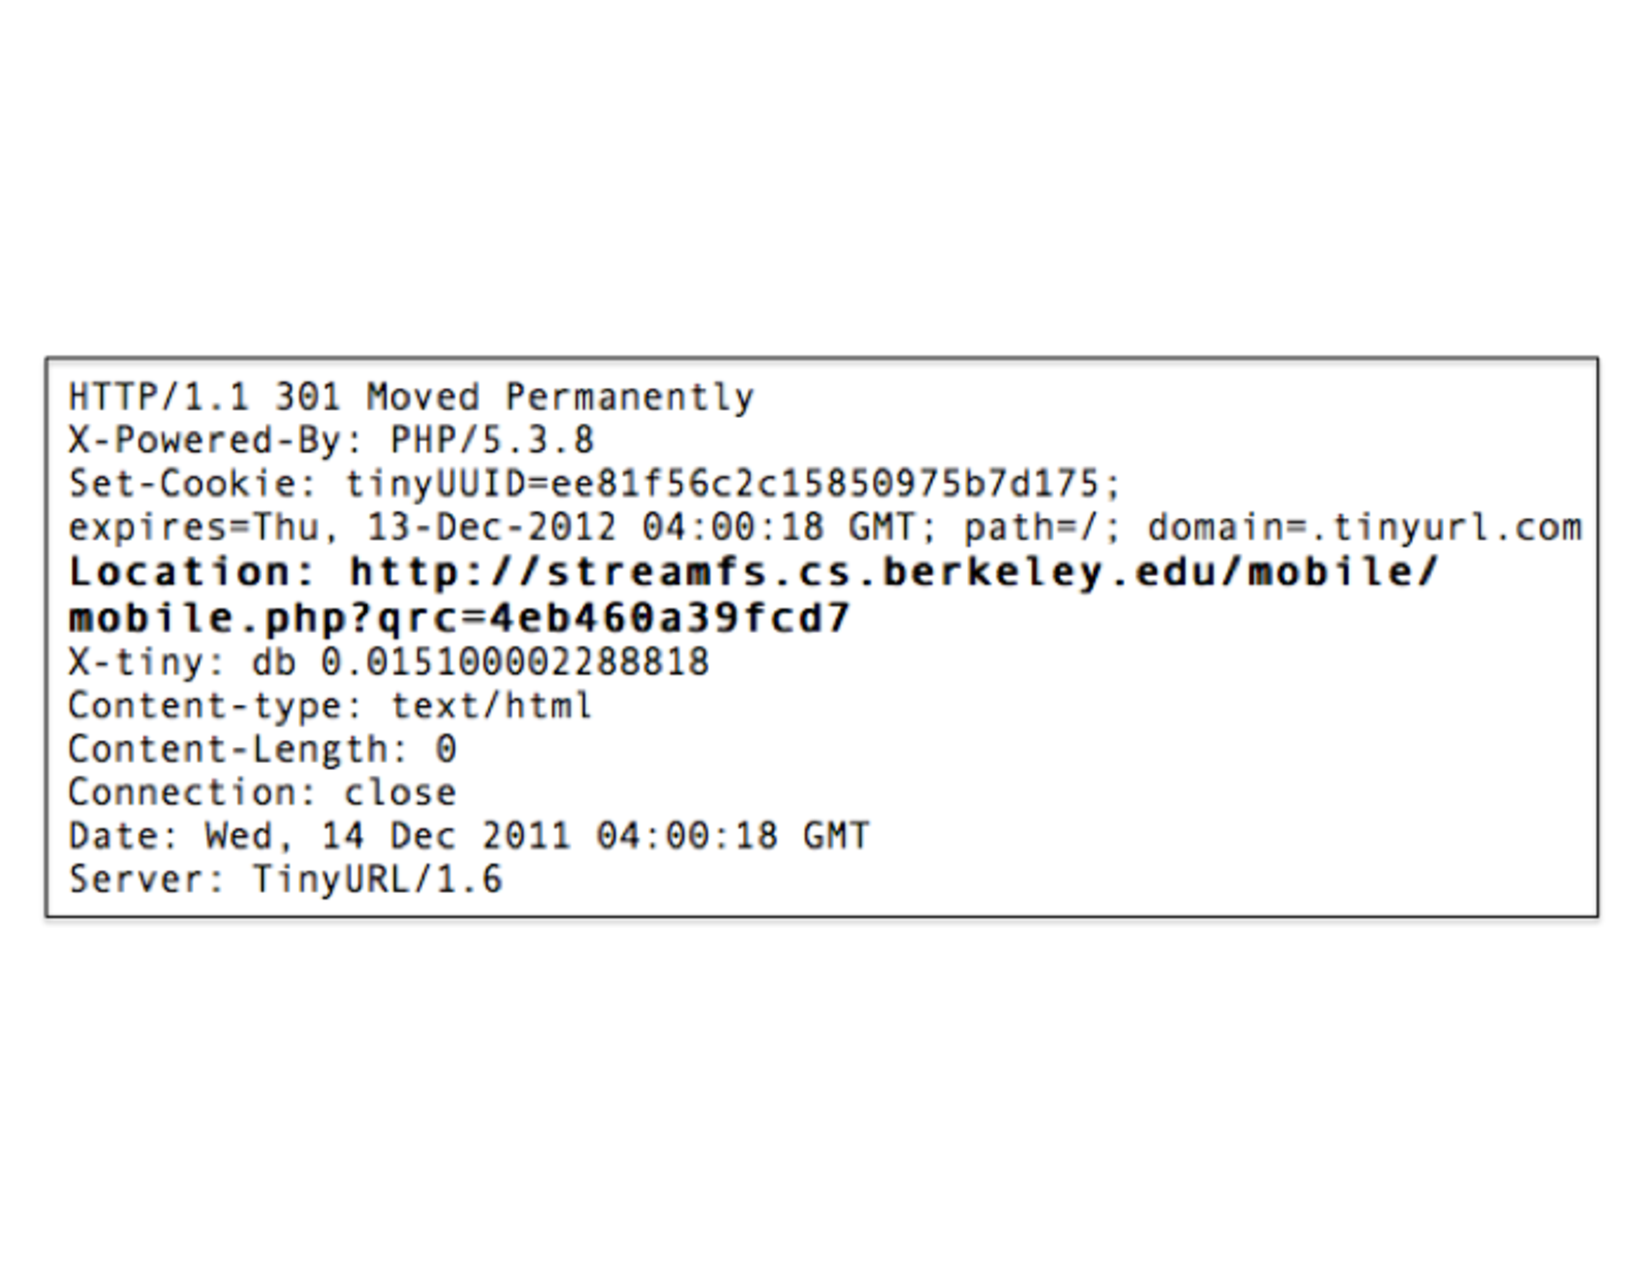
\includegraphics[scale=0.30]{figs/tinyurlhdr}
\caption{The header of the response from the \texttt{tinyUrl} when resolving a QR code.  The `Location' attribute
is used to extract the unique identifier for the object this QR code tags.  It is also used to re-direct
users without the phone application to a meaningful web address for the object.}
\label{fig:tinyurlhdr}
\end{center}
\end{figure}


Notice the `Location' attribute in the header.  This is the location of the re-direct.  This approach gives us
flexibility in several ways:

\begin{enumerate}
\item It allows us to encode less information in the QR code, decreasing its visual complexity; making it more
		robust across phones with different camera quality, poor lighting conditions, and shaky hands.
\item It allows the added layer of indirection to serve two versions of the applications:  the native application,
		where users can \emph{deeply explore} and edit the entities and their relationships and the \emph{shallow lookup}, 
		which re-directs the mobile phone to a read-only view of the item that was scanned -- such as a power trace or 
		a description.
\end{enumerate}


It provides a web address for users to re-direct to and find information and various read-only services for the object.  However, because
the \texttt{URL} also contains a unique identifier \emph{qrc}, it can be used to provide for sophisticated services and capabilities.
An example is the ability to change the virtual structure of inter-relationship between this object and other objects.  This
is demonstrated in our energy auditing application discussed in detail in section~\ref{sec:eaudit}.
Once items are tagged, they can be added and removed by swiping the tag and pressing the button for what you want to do with
the item.  You also check into locations either explicit with a location-tag swipe or implicitly with an item swipe.

\emph{Shallow} applications
use the \texttt{URL} directly.  The \emph{qrc} \texttt{URL} is unqiue identifier for the item that this tag is attached to.
A shallow application can obtain mostly read-only service through our web applications.  For example, we'll see how
to get either item-specific data or item-aggregated data with respect to the user making the request (i.e. the total
energy consumed by \emph{my} devices).  \emph{Deep-inspection} applications are native to the phone, so we can do much
more with the tag.  Our energy auditing application allows you to related the item to other items by maintaining state of swipe
history.  This is more difficult with the web-applicaiton.  We can also use the tag and item information to couple it with
sensor information coming from sensors on the phone itself.  For example, we could determine the direction an object
is pointing by using the phone's directional sensor and negating their direction (i.e. phone is facing east, tag on item must
be facing west).

\begin{figure*}[htb!]
\begin{center}
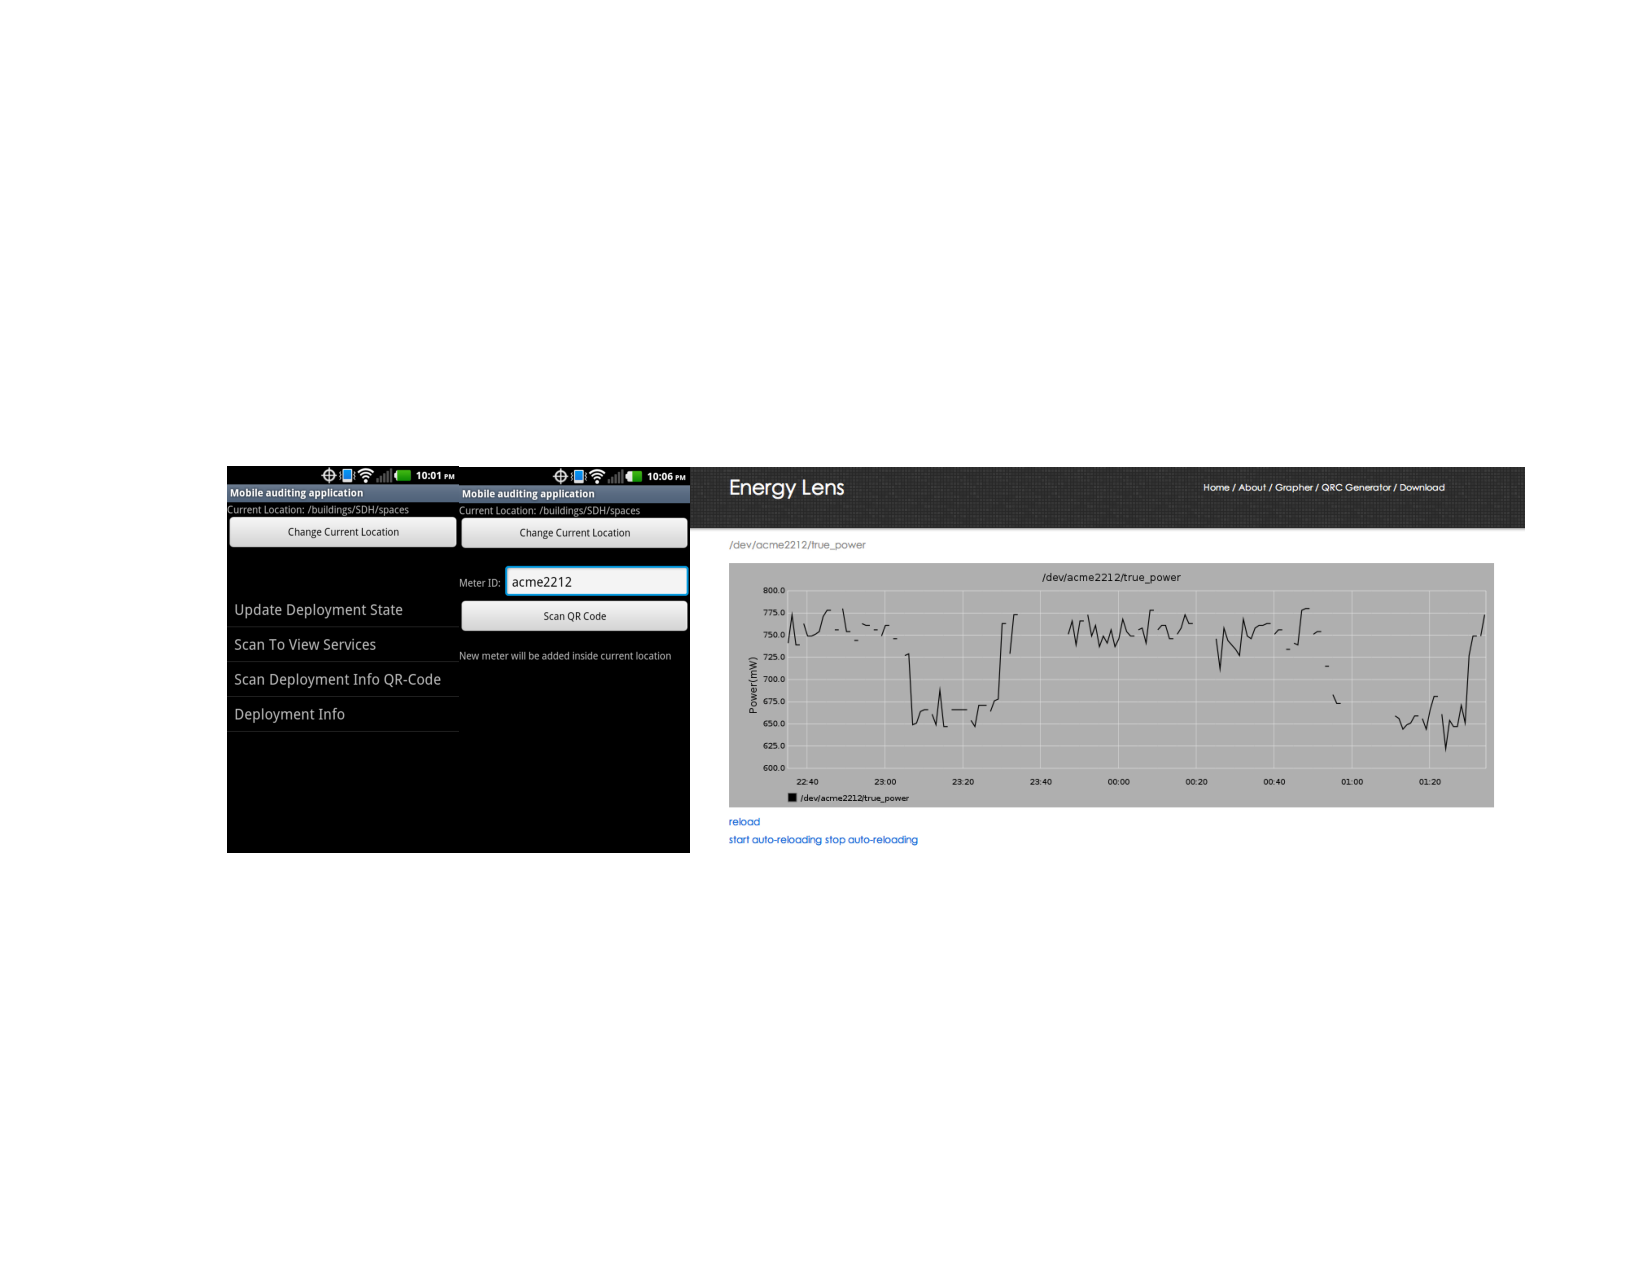
\includegraphics[width=\textwidth]{figs/mobileapp}
\caption{Screen shots of the mobile application.  The screens on the left are for editing the state of the deployment.
The graph on the right shows a live feed of a the sensor that's attached to the item that was scanned with the `Scan To
View Services' option in the mobile application.  It can also be resolved by scanning the QR code and following the re-direct
to the URL.}
\label{fig:mobileapp}
\end{center}
\end{figure*}

ACme meters are IP-enabled and forward their data through a router that runs sMAP.  sMAP then forwards the incoming data
to StreamFS, running in a machine in Amazon's EC2.  StreamFS is a web service that organizes streaming data and metadata using
a hierarchical naming convention.  It also provide a pub/sub facility for streaming data.  We construct 
a canonical naming convention within StreamFS to express the entity relationships between people, things, and meters.  The pub/sub
mechanism allows us to combine the ERG with streaming data, and feeds our timeseries data viewers.













\subsection{EnergyLens Evaluation}
\label{sec:eval}



% \subsection{Application layer}

% \begin{figure}[htb!]
% \begin{center}
% 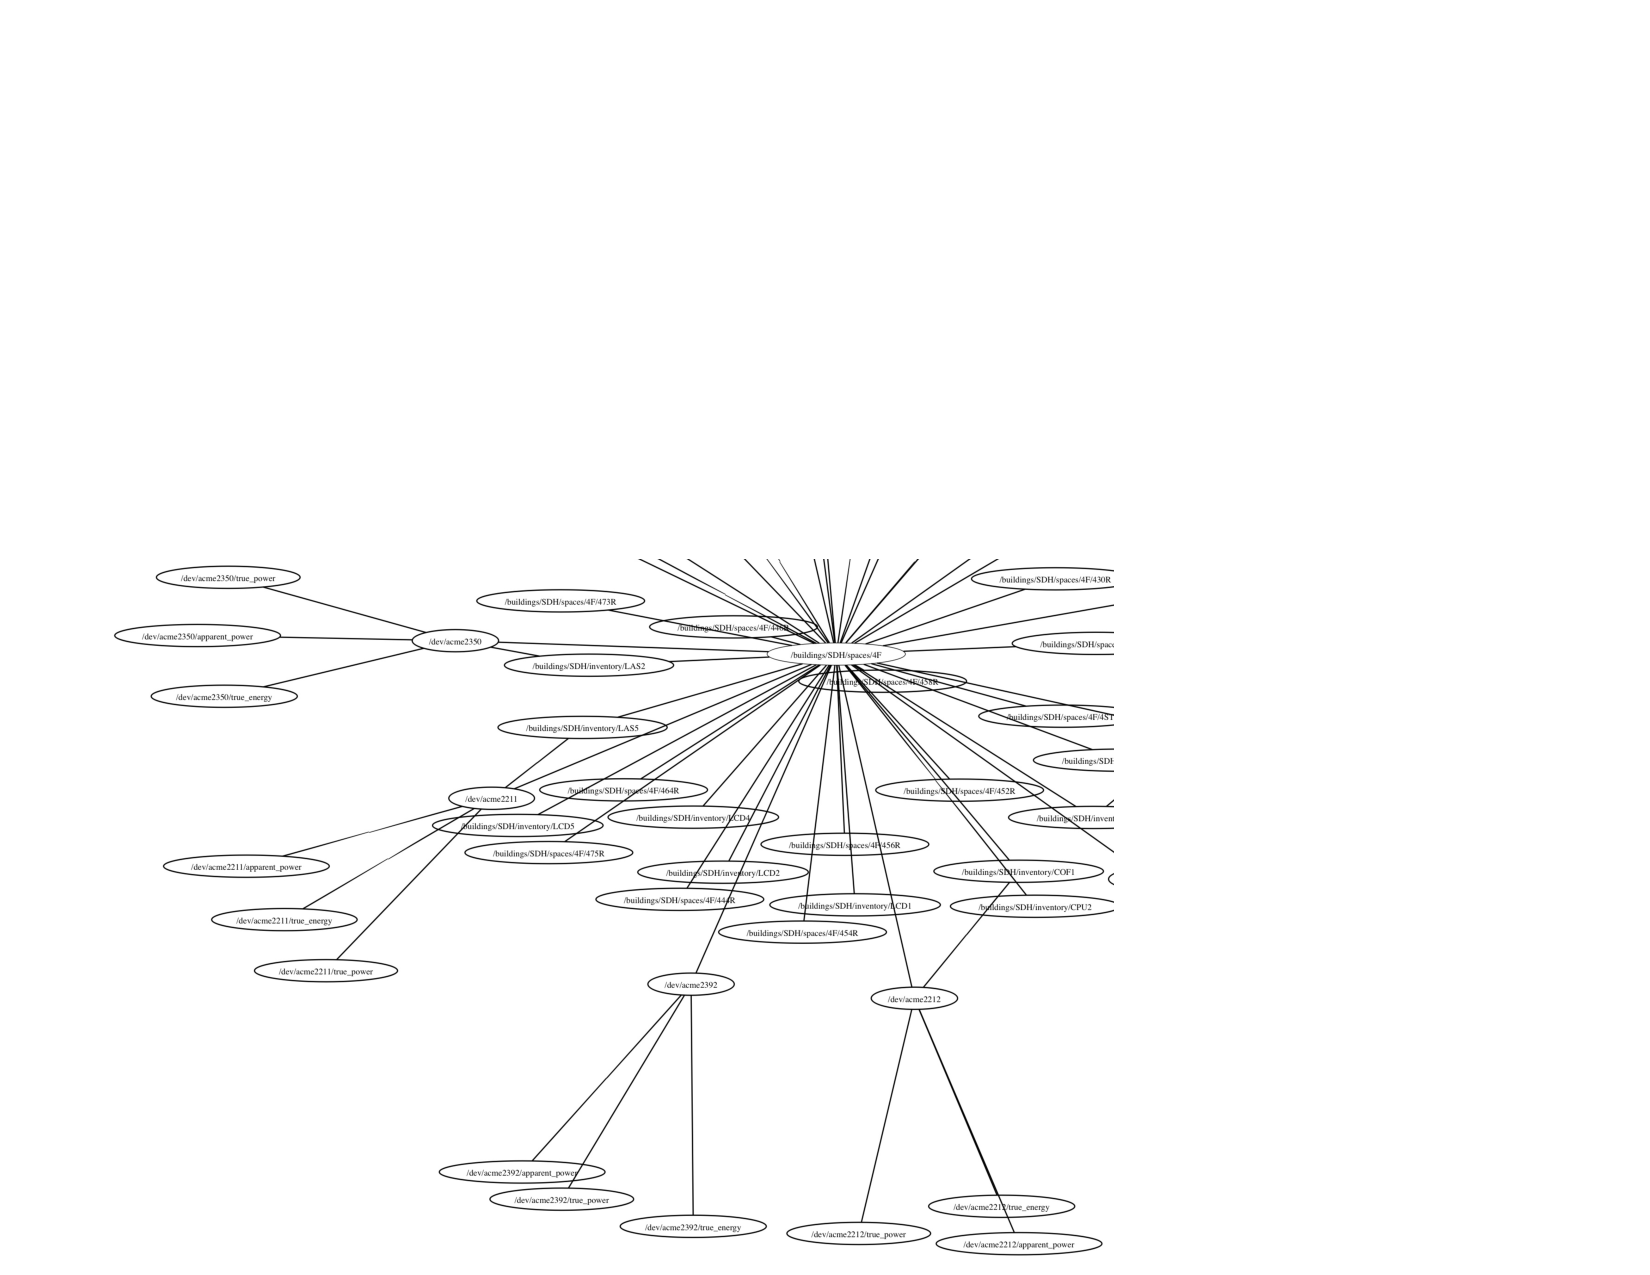
\includegraphics[scale=0.45]{figs/SDH_4F_ERG_closeup}
% \caption{A portion of the prefetched entities on the a single floor in our building.  This shows a snapshot of the entity-relationship
% graph for that floor.  Each node, link, and associated content is prefetched when the user swipes the floor
% tag or anything on that floor.}
% \label{fig:sdh_4f_erg}
% \end{center}
% \end{figure}


In this section we measure prefetch download times and discuss strategies for providing scalability.  We also
look at the transaction manager and discuss conflict resolution.

\begin{figure}[htb!]
\begin{center}
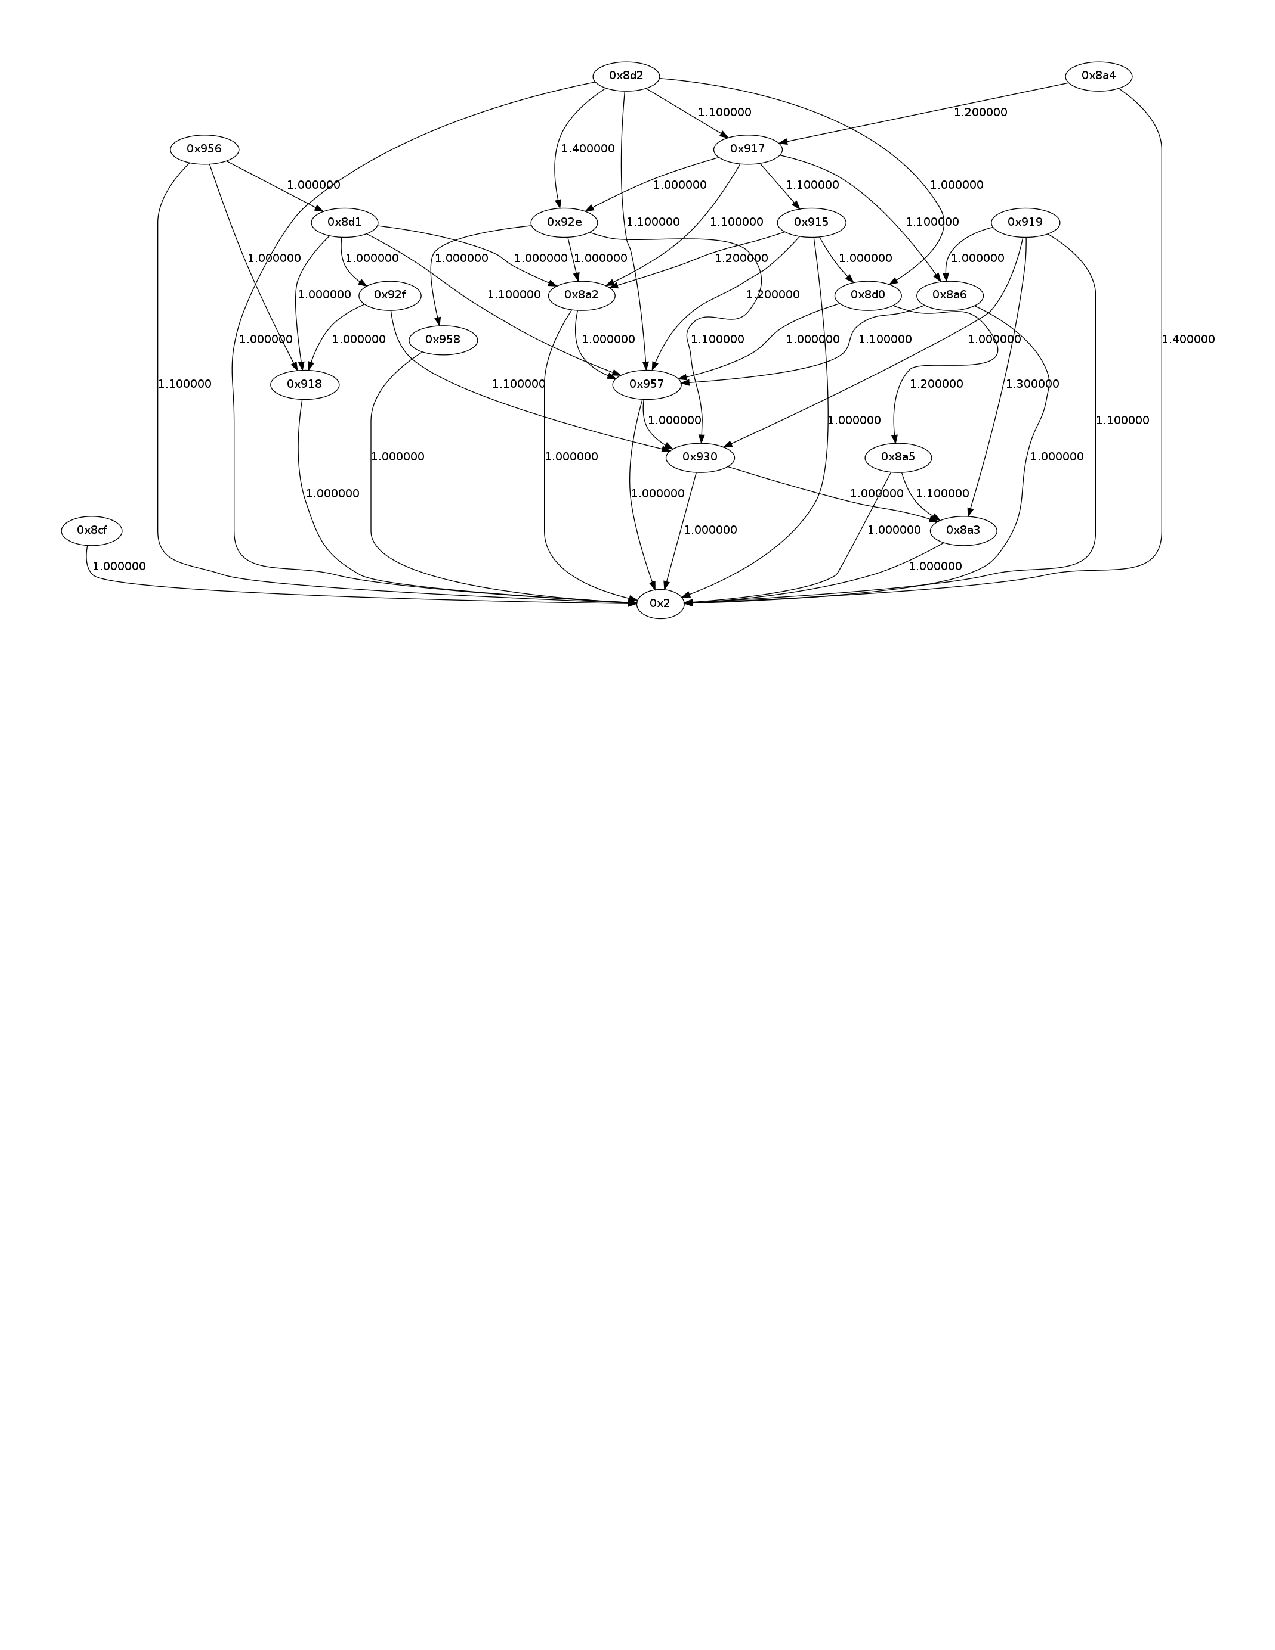
\includegraphics[scale=0.8]{figs/acmenetwork_SDH_4F}
\caption{}
\label{fig:acmenetwork_SDH_4F}
\end{center}
\end{figure}
\subsubsection{Sensing and tag layer}
% We deployed 20 ACme power meters~\cite{acmemeter} on a single floor of a building on campus.  The data was made available through
% sMAP~\cite{smap} and forwarded to our processing and data management layer, StreamFS.  We distributed
% the ACmes throughout a single floor in our building and registered various plug loads as being measured by them.  We also tagged
% hundreds of items and locations throughout the entire building.  In total we tagged 20 meters, 20 metered items, 351 un-metered items,
%  and 139 rooms over 7 floors. 

StreamFS supports the addition and operations to record all the deployment information.  It also supports active aggregates for 
31 rooms on the 4th floor of the deployment and 1 for the entire building.  The number of active users was no more than 10 at any time.
Because these number are not that large they do not truly test the scalability of the system.  However, they do demonstrate
both \emph{extensibility} and \emph{generalizability}.  Without the first property we could not have added the the sensors,
related information, user context, spatial configuration information and updated it with ease.  Without the second property
we could not have supported both the collection of metadata and data about the deployment as well as \emph{data services} that
are absolutely crucial to the success of the Energy Lens application.

Also, we used a single function and instantiated 32 instances of it in the deployment.  This demonstrate the \emph{ease of management}
property we set to provide through StreamFS.  Because we follow the principle where ``everything is a file'' the entire deployment
data, metadata, and analytics can be accessed and controlled from the same deployment.

\subsubsection{Prefetching}
Prefetching occurs when a user enters a new floor, as detected by a floor scan or an item
scan.  Table~\ref{tab:prefetchtimes} shows that the prefetch times scale linearly with the number of
items (and data) to prefetch.  Each node holds approximate 100 bytes or information and for
a 20-node deployment of power meters, producing 100 bytes of data per stream (three streams per ACme) every 20 seconds, we fetch 
approximately 1 MB of data.

These prefetch times are non-trivial to deal with, especially since they cause the phone application to slow down
until the data is received and loaded into the local cache.  The overhead is dominated by the query in StreamFS that 
constructs the entire sub graph to send to the application.  For future work,  we are will implement a
callback facility and pass the application a reference to it.  The app can then periodically check back until
the query completes and the data is ready to be downloaded.  We can also include partial responses to the query
in the prefetch-loop response.  This also allows users to continue using the application without any frustrating waits.

\subsubsection{Log dump measurements}
\begin{table}
\begin{center}
  \begin{tabular}{| r | c  c | }
    \hline
    \textbf{No. nodes} & \textbf{Fetch time (sec)} & \textbf{Std. Error (sec)} \\ \hline
    1       &   0.8902      & 0.0756 \\ \hline
    10      &   5.7342      & 1.7087 \\ \hline
    100     &   52.3145     & 14.1146 \\ 
    \hline
  \end{tabular}
\caption{Shows the time to fetch nodes based on the size of the fetch.  The fetch time
increased linearly with the number of nodes.  Caching maintain fetch time near
that of fetching a single node.  A callback is used when cache is invalidated.}
\label{tab:prefetchtimes}
\end{center}
\end{table}


% \subsubsection{Log replay latency}
Table~\ref{tab:optimes} shows the  operations that the transaction manager calls on the StreamFS server.
Log replay and transaction processing is entirely dependent on the time to execute these operations on StreamFS.
There are five types of transactions, a \emph{move}, a \emph{un/bind}, \emph{un/attach}.  A move is a combination
of a `delete' and a `create link', a bind is a `create link' and an `update tags', an unbind and unattach is a
`delete' and `update tag'.  The transaction latency is the sum of these operations.  By far the most expensive
operation is a `create node' operation.  This occurs when a user adds a new item/space/person to the graph.
The time to apply the operation also scales linearly with the size of the logs.  

All logs dumps are processed sequentially.  However, for future work we look to parallelize processing into
parallel processes updating different portions of the graph.  For example, log updates rooted at different floors
could occur simultaneously.

The global transaction manager implements three main high-level operations -- rollback, apply, and replay.  Our current implementation
is limited by the time is takes to perform an operation on StreamFS.  Table~\ref{tab:optimes} shows the three 
main operation that the transaction manager needs to do on the server.
% Maybe we include another table that talks about the trace we ran through and the conflict times, etc.

Usually rollbacks consist of \emph{delete} operation and applies consist of \emph{creates}.  In a worst-cases analysis
of performance we expect the total conflict resolution time to be roughly bounded by
$rollback\_time + apply\_time + replay\_time$, since $replay\_time=3 X rollback\_time$ and apply\_time is negligible, 
the total time is approximately $4 X rollback\_time$.  Therefore the overhead is driven by how many new links were created
that have to be deleted and then re-created.  As an optimization, we limit the scope of a rollback.  The naive
approach is to blindly undo all operations up to a certain time.  However, we can use the location of the node
in the ERG to limit the conflict-scope to a sub graph, rather than the entire graph.  The simplest approach is to check if the operation
on a node either shares an immediate parent with the node that will have an operation undone on it or it the operation
is on the same node.  By limiting conflict-scope we minimize the number of operation that get execute and, hence, minimize the 
cost of resolution.


\begin{table}
\begin{center}
  \begin{tabular}{| l | c  c | }
    \hline
    {\textbf Operation } & {\textbf Avg. exec. time (ms) } &\\ \hline
    fetch & 250 &\\ \hline
    delete & 326  &\\ \hline
    update tags & 267  &\\ \hline
    create link & 250  &\\ \hline
    create node & 1036  &\\ 
    \hline
  \end{tabular}
\caption{Average operation execution time in StreamFS.}
\label{tab:optimes}
\end{center}
\end{table}

% \begin{itemize}
% \item Forwarding
% \item Conflict resolution
% \end{itemize}




% The main driver for the EnergyLens work is to explore the fundamental challenges related to:

% \begin{enumerate}
% \item Tracking people and objects.
% 	\begin{itemize}
% 	\item Through local crowd-sourcing of the tasks to building occupants
% 	\end{itemize}
% \item Maintaining consistency between the relationship between physical items and the entity-relationship graph that represents it.
% \item Providing real-time statistics, information, and processing of energy data related to the building environment.

% 	\begin{itemize}
% 	\item With respect to the occupants
% 	\item with respect to spaces
% 	\item Maintaining security and privacy
% 		\begin{itemize}
% 		\item specifically with respect to personal data and control
% 		\end{itemize}
% 	\end{itemize}

% \end{enumerate}






